\documentclass[14pt,a4paper]{scrartcl}
\usepackage[utf8]{inputenc}
\usepackage[english,russian]{babel}
\usepackage{misccorr,color,ragged2e,amsfonts,amsthm,graphicx,systeme,amsmath,mdframed,lipsum}
\renewcommand\qedsymbol{$\blacksquare$}
\renewcommand*{\proofname}{\text{Доведення}}
\theoremstyle{definition}
\newtheorem{defo}{Означення}[section]
\newtheorem*{teo}{Теорема}
\newtheorem*{example}{Приклад}
\theoremstyle{remark}
\newtheorem*{remark}{Зауваження}
\theoremstyle{definition}
\newtheorem*{consequence}{Наслідок}
\theoremstyle{definition}
\newtheorem{statement}{Утверждение}[section]
\newmdtheoremenv{boxteo}{Теорема}[section]
\setlength\parindent{0pt}
\DeclareMathOperator*\lowlim{\underline{lim}}
\DeclareMathOperator*\uplim{\overline{lim}}
\begin{document}


\def\be{\begin{equation}}
\def\ee{\end{equation}}

\def\bd{\begin{defo}}
\def\ed{\end{defo}}

\def\bbt{\begin{boxteo}}
\def\ebt{\end{boxteo}}
\begin{center}
  Розрахункова робота №4\\
  студента КА-96\\
  Терещенка Дениса\\
  Варіант-26\\
\end{center}

\textbf{1.26} Дослідити на збіжність ряд.

$$  \sum\limits_{n = 1}^{ \infty}{ \frac{3 + 7n}{5^n+n} } $$
Скористаємося ознакою Даламбера: $$ \lim\limits_{n\to  \infty}{ \frac{a_{n+1}}{a_n} } =  \lim\limits_{n\to  \infty}{ \frac{  \frac{10 + 7n}{5*5^n + n + 1}  }{ \frac{3 + 7n}{5^n+n}  } } =
 \lim\limits_{n\to  \infty}{
  \frac{5^n*n*(1 + \frac{n}{5^n} )(7+10/n)}{5^n*n*(5 + \frac{n+1}{5^n} )(7 + 3/n) }
} = \left| \begin{gathered}
  \frac{n}{5^n} \to 0 \quad \frac{n+1}{5^n} \to 0\\
  3/n \to 0 \quad 10/n \to 0\\
\end{gathered} \right| =
 $$
 $
= 0.2 < 1
 $  - тому за ознакою Даламбера ряд $ \sum\limits_{n = 1}^{ \infty}{\frac{3 + 7n}{5^n+n} }$ - збіжний.


\textbf{2.26} Знайти область збіжності функціонального ряду.\\
$$  \sum\limits_{n = 1}^{ \infty}{\frac{\left| x \right|^n  + \left| x \right|^{-n}} {2}} $$
Застосуємо радикальна ознака Коши для $\left| a_n \right|$ :\\
$$
 \uplim\limits_{n\to  \infty}{ \sqrt[n] { \left| a_n \right|  }} =
  \uplim\limits_{n\to  \infty}{ \sqrt[n]{ \left| \frac{\left| x \right|^n  + \left| x \right|^{-n}} {2} \right|  } } = \left| x \right|
$$
Тоді ряд є абсолютно збіжним за умови $ \left| x \right| < 1  \Leftrightarrow x \in (-1, 1)$
\\
Із зауваження до ознак Даламбера і Коші: $ x \in (- \infty; -1) \cup (1; \infty)$ - ряд є розбіжним. Розглянемо точки $x=1, x= -1:$
$$
x=-1 : \qquad  \sum\limits_{n = 1}^{ \infty}{ \frac{1+1}{2} } - \text{розбіжний}
$$
$$
x=1 : \qquad  \sum\limits_{n = 1}^{ \infty}{ \frac{1+1}{2} } - \text{розбіжний}
$$
Остаточно: $x \in (-1; 1) $ - абсолютно збіжний. \\
$ x \in (- \infty; -1] \cup [1; \infty)$ - розбіжний.\\

\pagebreak

\textbf{3.26} Знайти область збіжності функціонального ряду.\\

$$  \sum\limits_{n = 1}^{ \infty}{ \frac{2^n}{n^4} \sin^n{(3x)}  }  \Rightarrow a_n = \frac{2^n}{n^4}\sin^n{(3x)}  $$
Дослідимо абсолютну збіжність(за ознакою Коші): $  \uplim\limits_{n\to  \infty}{ \sqrt[n]{\left| a_n \right|} } =  \uplim\limits_{n\to  \infty}{  \sqrt[n]{ \left|\frac{2^n}{n^4}\sin^n{(3x)}    \right| }  } =  \sqrt[n]{ \left|\frac{2^n}{n^4}\sin^n{(3x)}    \right| }  =  \left| 2 \sin{(3x)}  \right| \Rightarrow 2 \left| \sin{(3x)}  \right| < 1 $ - ряд абсолютно збіжний.\\
Перевіримо у крайніх точках(де $ \left| \sin(3x) \right|  $):\\
$$\frac{2^n}{n^4} > 0 \Rightarrow \left| a_n \right| = \left| \frac{2^n}{n^4}\sin{(3x)}   \right| =  \frac{2^n}{n^4} \left| \sin{(3x)}  \right| $$
Підставимо
$ \left| \sin{(3x)}  \right| = 1/2 \Longrightarrow |a_n| = \frac{2^n}{n^4} * \frac{1}{2^n } \Longrightarrow $ Озн. порівняння в границях з еталонним $\frac{1}{n^4}   \Longrightarrow  \lim\limits_{n\to  \infty}{ \frac{ \frac{1}{n^4} }{  \frac{1}{n^4} } } = 1 \Rightarrow$ Ряд збігається абсолютно при $\sin{(3x)} = \pm 1/2 $. \\

Розв'яжемо тригонометричне рівняння: $ \left| \sin{(3x)}  \right| \leq 1/2  \Leftrightarrow  \left\lbrace \begin{gathered}
\sin{(3x)} \leq  1/2\\
\sin{(3x)} \geq -1/2\\
\end{gathered} \right. \Leftrightarrow $

\begin{center}
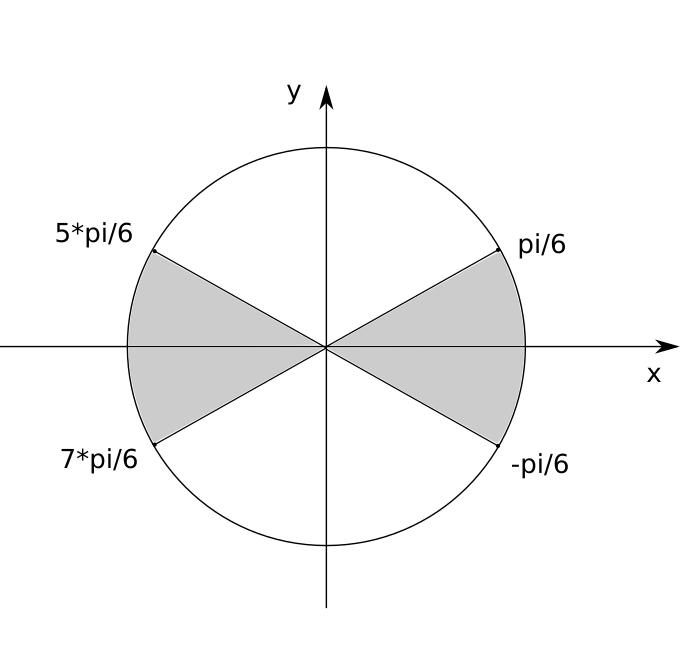
\includegraphics[scale=0.4]{im1}
\end{center}
$$
\Leftrightarrow \left[ \begin{gathered}
     \frac{-\pi}{6} + 2n\pi \leq 3x \leq \frac{\pi}{6} + 2n\pi\\
      \frac{7\pi}{6} + 2n\pi \leq 3x \leq \frac{5\pi}{6} + 2n\pi
\end{gathered} \right.
\Leftrightarrow \left[ \begin{gathered}
     \frac{-\pi}{18} + 2n\pi/3 \leq x \leq \frac{\pi}{18} + 2n\pi/3\\
      \frac{7\pi}{18} + 2n\pi/3 \leq x \leq \frac{5\pi}{18} + 2n\pi/3
\end{gathered} \right.
$$
Остаточно запишемо: ряд $\sum\limits_{n = 1}^{ \infty}{ \frac{2^n}{n^4} \sin^n{(3x)}  }$ є абсолютно збіжним при\\ $\frac{-\pi}{18} + n\pi/3 \leq x \leq \frac{\pi}{18} + n\pi/3, n\in \mathbb{Z}$. За зауваженням до признаків Коші та Даламбера на решті проміжку $ \frac{\pi}{18} + \frac{n\pi}{3} \leq x \leq \frac{5\pi}{18} + \frac{n\pi}{3}, n\in \mathbb{Z}    $ ряд є розбіжним.

\textbf{4.26} Для заданого функціонального ряду побудувати мажоруючий ряд
та довести рівномірну збіжність на вказаному відрізку.\\
$$  \sum\limits_{ n = 1}^{ \infty}{\sin{( \frac{\pi}{2^n} )}(x-2)^n } \qquad [1;3]$$
Використаємо признак Вейерштрасса. На заданому відрізку виконується: $ \left| x-2  \right| \leq 1 $. Тоді:\\
$$
\left| a_n \right| = \left| \sin{( \frac{\pi}{2^n} )} (x-2)^n  \right| \leq   \sin{( \frac{\pi}{ 2^n} )} * 1^n \leq \sin{( \frac{\pi}{2^n} )} - \text{І умова озн. В.}
$$
Доведемо збіжність ряду $  \sum\limits_{n = 1}^{ \infty}{ \sin{( \frac{\pi}{2^n} )} } \sim  \sum\limits_{n = 1}^{ \infty}{ \frac{\pi}{2^n} }$ \\
$  \uplim\limits_{n\to  \infty}{ \sqrt[n]{ \frac{\pi}{2^n} }} =  1/2 $ $\Rightarrow$ Збіжний за озн. Коши. - 2-га умова ознаки Вейерштрасса.\\
Отже, за ознакою Вейерштрасса ряд є рівномірно збіжним на проміжку $[1,3]$. \\

\textbf{5.26} Знайти суму ряду.

$$
S(x) =  \sum\limits_{n = 2}^{ \infty}{ \frac{x^n}{ n(n-1)} } =  \sum\limits_{n = 2}^{ \infty}{ \frac{x^n}{n-1} -  \sum\limits_{n = 2}^{ \infty}{ \frac{x^n}{n} } } = S_1(x) - S_2(x)
$$
Використаємо властивості почленного інтегрування та дифференціювання суми ряду на області збіжності.
$$
S_1(x) = x  \sum\limits_{n = 2}^{ \infty}{  \frac{x^{n-1}}{n-1} } = x \tilde{S_1}(x)
$$
Зауважемо, що отримали суму нескінченої геом. прогресії:
$$
\tilde{S_1}'(x) =  \sum\limits_{n = 2}^{ \infty}{x^{n-2}} = \frac{1}{x^2}  \sum\limits_{n = 2}^{ \infty}{x^n} = \frac{1}{x^2} * \frac{x^2}{1-x} = \frac{1}{1-x}
$$
$$
\tilde{S_1}(x) =  \int\limits_{0}^{x}{ \frac{1}{1-x}dx } = - \ln{(1-x)} \Rightarrow S_1(x) = -x \ln{1-x}
$$

$$
S_2(x) =  \sum\limits_{n = 2}^{ \infty}{ \frac{x_n}{n} } \qquad S'_2(x) =  \sum\limits_{n = 2}^{ \infty}{x^{n-1} } = \frac{x}{1-x} \Rightarrow S_2(x) =  \int\limits_{0}^{x}{ \frac{x}{1-x}dx }  = - \ln{(1-x)} - x
$$
\textbf{Таким чином, отримали:} $S(x)= x + \ln{(1-x)} - x \ln{(1-x)} $. \\

\textbf{6.26} Розкласти функцію в ряд Тейлора за степенями x.\\
$$
f(x) = \frac{5}{6-x-x^2} =  \frac{-5}{ (x+3)(x-2)}
$$
За методом невизначених коефіцієнтів:
$$
f(x) = \frac{1}{x+3} - \frac{1}{x-2} =  \frac{1}{3(1+ \frac{x}{3} )} + \frac{1}{2(1 - \frac{x}{2} )}
$$
За розкладом $\frac{1}{1+x} = 1- x +x^2 + ...$\\
Отже, $f(x) = \frac{1}{3} ( 1 - x/3 + x^2/9 - x^3/27 + ... + (-1)^n* ( \displaystyle\frac{x^n}{3^n}  )+...) $ + $ \frac{1}{2} (1 + \frac{x}{2} + \frac{x^2}{4} + ... + \displaystyle \frac{x^2}{2^n}  +... ) = $
$$= \frac{5}{6} + \frac{5}{36}x + ... + \left( \frac{1}{2^{n+1}} +  \frac{(-1)^n}{3^{n+1}}   \right)x^n+ ...    $$

\textbf{7.26} Обчислити інтеграл з точністю до 0,001.\\

$$
 \int\limits_{0}^{0.5}{\frac{1}{\sqrt[3]{1+x^3}} }
$$
Розкладемо: $ \frac{1}{\sqrt[3]{1+x^3}} =  1 - \frac{x^3}{3} + \frac{2}{9}x^6 - \frac{14}{81}x^9 + \frac{35}{243}x^{12} - ...  $\\
За властивістю почленного інтегрування степеневого ряду, отримаємо:\\
$$
 \int\limits_{0}^{0.5}
 {\frac{1}{\sqrt[3]{1+x^3}} } =
 x \bigg|_{0}^{0.5} -
 \frac{x^4}{12}\bigg|_{0}^{0.5}
 + \frac{2}{63} x^7 \bigg|_{0}^{0.5}
 - \frac{7}{405} x^{10} \bigg|_{0}^{0.5}
 + \frac{35}{3159}x^{13}\bigg|_{0}^{0.5} - ... =
$$
$$
= 0.5 - \frac{2^{-4}}{12} + \frac{2^{-6}}{63} - \frac{7}{405}*2^{-10} + \frac{35}{3159} 2^{-13}- ...
$$
Цей знакопочерговий ряд задовільняє ознаки Лейбниця
(знакопочерговий ряд, $a_n \geq 0 \quad  \lim\limits_{n\to  \infty}{a_n} = 0$)
, тому з наслідку до озн. Лейбниця маємо:
$ \left| S - S_k \right| \leq a_{k+1} $.\\
Обчисливши перші члени ряду, маємо: $ a_3< 0.001 \Rightarrow k=2 \Rightarrow  \int\limits_{0}^{0.5}{\frac{1}{\sqrt[3]{1+x^3}} } \approx 0.5 - 0.005208 \approx 0.495 $ \\
\pagebreak\\
\textbf{8.26} Дослідити на збіжність ряд.\\
$$
 \sum\limits_{n = 2}^{ \infty}{ \frac{n}{(n^2)\ln{(n)}} }
$$
Спочатку порівняємо заданий ряд з рядом $  \sum\limits_{n = 2}^{ \infty}{ \frac{1}{n \ln{n}} }$.
$$
 \lim\limits_{n\to  \infty}{ \frac{\frac{n}{(n^2)\ln{(n)}}}{\frac{1}{n \ln{n}}} } = 1 \neq 0 \neq \infty
$$
А отже, за ознакою порівняння в границях обидва ряди збігаються або розбігаються одночасно. Дослідимо на збіжність ряд $ \sum\limits_{n = 2}^{ \infty}{ \frac{1}{n \ln{n}} }$. Скористаємося інтегральною ознакою Коші:\\
1. $a_n = \frac{1}{n \ln{n}}>0$\\
2. $f(x) = \frac{1}{n \ln{n}}, x\in [2, \infty] \quad f(n) = a_n \quad \forall n\geq 1$\\
3. $f(x) $ - монотонно спадає, а одже:\\
Ряд $ \sum\limits_{n = 2}^{ \infty}{ \frac{1}{n \ln{n}} }$ та $ \int\limits_{2}^{ +\infty}{ \frac{1}{x \ln{x}} }$ збігаються або розбігаються одночасно.\\
Дослідимо на збіжність інтеграл:
$$
 \int\limits_{2}^{ \infty}{ \frac{1}{x \ln{x}} } = \left| \begin{gathered}
   t = t(x)= \ln{x} \\
   dt = \frac{1}{x}dx\\
 \end{gathered}\quad \begin{gathered}
   t(2) = \ln{2}\\
   t(\infty) = \infty\\
 \end{gathered} \right| =  \int\limits_{ \ln{2}}^{ \infty}{ \frac{dt}{t} }
$$
Інтеграл є розбіжним, оскільки показник $t = 1$. З інтегральної ознаки Коші випливає, що ряд $  \sum\limits_{n = 2}^{ \infty}{ \frac{1}{n \ln{n}} } $ є розбіжним, а одже і \textbf{початковий ряд розбігається} за ознакою порівняння в границях.

\pagebreak
Допустим, некий обьект находится в координате O(x, y)\\ и имеет скорость $\vec{u}(u_x, u_y)$ \\
Существует некая цель - $T(x_t, y_t)$. \\Нужно направить скорость обьекта в сторону цели не изменив её модуль.\\
Пусть результирующая скорость: $\vec{v}(v_x, v_y)$.\\
Модуль скорости сохраняется, иначе: $ \left| \vec{v} \right| = \left| \vec{u} \right| \qquad v_x^2 + v_y^2 = u_x^2 + u_y^2    $
\end{document}
